\documentclass[9pt,twocolumn,twoside]{pnas-new}

\usepackage{gensymb}

% new commands
% q value
\newcommand{\qval}[1]{$q<10^{-#1}$}

% species names
\newcommand{\cel}{\emph{C.~elegans}}
\newcommand{\dicty}{\emph{D.~discoideum}}
\newcommand{\ecol}{\emph{E.~coli}}

% gene names
\newcommand{\gene}[1]{\mbox{\emph{#1}}}

\newcommand{\nlp}{\gene{nlp-31}}
\newcommand{\ftna}{\gene{ftn-1}}
\newcommand{\ftnb}{\gene{ftn-2}}
\newcommand{\cysl}{\gene{cysl-1}}
\newcommand{\nog}{\gene{nog-1}}
\newcommand{\nhr}{\gene{nhr-57}}
\newcommand{\lam}{\gene{lam-3}}
\newcommand{\fog}{\gene{fog-2(lf)}}
\newcommand{\egl}{\gene{egl-9(lf)}}
\newcommand{\rhy}{\gene{rhy-1(lf)}}
\newcommand{\vhl}{\gene{vhl-1(lf)}}
\newcommand{\eglvhl}{\gene{egl-9(lf);vhl-1(lf)}}
\newcommand{\eglhif}{\gene{egl-9(lf) hif-1(lf)}}
\newcommand{\hif}{\gene{hif-1(lf)}}

% protein names
\newcommand{\eglp}{EGL-9}
\newcommand{\rhyp}{RHY-1}
\newcommand{\nogp}{NOG-1}
\newcommand{\vhlp}{VHL-1}
\newcommand{\hifp}{HIF-1}
\newcommand{\fogp}{FOG-2}
\newcommand{\nhrp}{NHR-57}
\newcommand{\lamp}{LAM-3}
\newcommand{\cyslp}{CYSL-1}

% DE genes numbers:
\newcommand{\egln}{2,549}
\newcommand{\rhyn}{3,005}
\newcommand{\vhln}{1,275}
\newcommand{\eglvhln}{3,654}
\newcommand{\hifn}{1,075}
\newcommand{\eglhifn}{744}
\newcommand{\fogn}{2,840}
\newcommand{\total}{7,609}

% downstream targets
\newcommand{\egltargets}{4}
\newcommand{\rhytargets}{0}
\newcommand{\vhltargets}{71} % 72 minus vhl-1 (IDed due to deletion)
\newcommand{\hiftargets}{312}
\newcommand{\hifohtargets}{56}

% website commands
\newcommand{\website}{
            \url{https://wormlabcaltech.github.io/mprsq/}
            }
\newcommand{\webref}{
\href{https://wormlabcaltech.github.io/mprsq/}{website}}

\templatetype{pnasresearcharticle} % Choose template

\title{Reconstructing a metazoan genetic pathway with transcriptome-wide epistasis
       measurements}

\author[a, b, 1]{David Angeles-Albores}
\author[a, b, c, 1]{Carmie Puckett Robinson}
\author[a]{Brian A. Williams}
\author[a]{Barbara J. Wold}
\author[a, b]{Paul W. Sternberg}

\affil[a]{Division of Biology and Biological Engineering, Caltech, Pasadena, CA,
          91125, USA}
\affil[b]{Howard Hughes Medical Institute, Caltech, Pasadena, CA, 91125, USA}
\affil[c]{Department of Neurology, Keck School of Medicine, University of
          Southern California, Los Angeles, California, 90033, USA}

% Please give the surname of the lead author for the running footer
\leadauthor{Angeles-Albores}

% Please add here a significance statement to explain the relevance of your work
\significancestatement{Transcriptome profiling is a way to quickly and
quantitatively measure gene expression level. Because of their quantitative
nature, there is widespread interest in using transcriptomic profiles as a
phenotype for genetic analysis. However, a source of major concern is that
whole-animal transcriptomic profiles mix the expression signatures of multiple
cellular states, making it hard to accurately reconstruct genetic interactions.
Additionally, it has been difficult to quantify
epistasis, the signature of genetic interaction between two genes, in these
molecular phenotypes. Here, we show that it is possible to accurately
reconstruct genetic interactions between genes using whole-animal RNA
sequencing, and we demonstrate a powerful new way to measure and understand
epistasis arising from these measurements. This suggests that whole-organism
RNA-seq can be a powerful tool with which to understand genetic interactions in
entire organisms and not only in isolated cells. With the advent of genome
engineering tools, generating mutants has become easier and faster for many
organisms. As mutants become easier to create, phenotyping them has become a
major bottleneck in understanding the biological functions of the genes in
question. Our work presents a possible solution to this problem, because
transcriptome profiling is fast and sensitive to genetic perturbations regardless
of the context they operate in.
}

% Please include corresponding author, author contribution and author declaration information
\authorcontributions{DAA, CPR and PWS designed experiments. CPR handled strains
and extracted RNA.\@ BAW generated RNA-seq libraries. BJW provided resources.
DAA, CPR and PWS wrote the paper.}
\authordeclaration{The authors declare no conflict of interest.}
\equalauthors{\textsuperscript{1} DAA  and CPR contributed equally to this work.}
\correspondingauthor{\textsuperscript{2}To whom correspondence should be
                     addressed. E-mail: pws@caltech.edu}

% Keywords are not mandatory, but authors are strongly encouraged to provide
% them. If provided, please include two to five keywords, separated by the pipe
% symbol, e.g:
\keywords{Epistasis $|$ Genetic Interaction $|$ Transcriptome $|$ Hypoxia}

\begin{abstract}
RNA-seq is commonly used to identify genetic modules that respond to
perturbations. In single cells, transcriptomes have been used as phenotypes, but
this concept has not been applied to whole-organism RNA-seq. Linear models can
quantify expression effects of individual mutants and identify epistatic effects
in double mutants. To make interpretation of these high-dimensional measurements
intuitive, we developed a single coefficient to quantify transcriptome-wide
epistasis that accurately reflects the underlying interactions. To demonstrate
our approach, we sequenced four single and two double
\emph{Caenorhabditis~elegans} mutants. From these mutants, we reconstructed the
known hypoxia pathway. In addition, we uncovered a class of \hifohtargets{}
genes that have opposing changes in expression in \egl{} and \vhl{} but the
\eglvhl{} mutant has the same phenotype as \egl{}. These changes violate the
classical model of HIF-1 regulation, but can be explained by postulating a role
of hydroxylated HIF-1 in transcriptional control.

\end{abstract}

\dates{This manuscript was compiled on \today}
\doi{\url{www.pnas.org/cgi/doi/10.1073/pnas.XXXXXXXXXX}}

\begin{document}

% Optional adjustment to line up main text (after abstract) of first page with
% line numbers, when using both lineno and twocolumn options. You should only
% change this length when you've finalised the article contents.
\verticaladjustment{-2pt}

\maketitle
\thispagestyle{firststyle}
\ifthenelse{\boolean{shortarticle}}{\ifthenelse{\boolean{singlecolumn}}{\abscontentformatted}{\abscontent}}{}

\dropcap{G}enetic analysis of molecular pathways has traditionally been
performed through epistatic analysis. Generalized epistasis indicates that two
genes interact functionally; such interaction can involve the direct interaction
of their products or the interaction of any consequence of their
function~\cite{Huang2006}. If two genes interact, and the mutants of these genes
have a quantifiable phenotype, the double mutant of interacting genes will have
a phenotype that is not the sum of the phenotypes of the single mutants that
make up its genotype. Epistasis analysis remains a cornerstone of genetics
today~\cite{Phillips2008}.

Recently, biological studies have shifted in focus from studying single
genes to studying all genes in parallel. In particular,
RNA-seq~\cite{Mortazavi2008} enables biologists to
identify genes that change expression in response to a perturbation.
% Gene expression
% profiling using RNA-seq has become much more sensitive thanks to deeper and more
% frequent sequencing due to lower sequencing costs~\cite{Metzker2010},
% better and faster abundance quantification~\cite{Patro2014,Bray2016,Patro2015},
% and improved differential expression analysis
% methods~\cite{Pimentel2016,Trapnell2013}.
RNA-seq has been successfully used to identify genetic modules involved in a
variety of processes, such as in the \emph{Caenorhabditis~elegans} linker cell
migration~\cite{Schwarz2012}, and planarian stem cell
maintenance~\cite{VanWolfswinkel2014,Scimone2014}. For the most part, the role
of transcriptional profiling has been restricted to target gene identification,
and so far there are only a few examples where transcriptomes have been used to
generate quantitative genetic models of any kind. In population genetics, eQTL
studies have established the power of transcriptomes for genetic
mapping~\cite{Brem2002,Schadt2003,Li2006,King2014}. Genetic pathway analysis via
epistasis has only been performed once in
\emph{Saccharomyces~cerevisiae}~\cite{Hughes2000} and once in
\emph{Dictyostelium~discoideum}~\cite{VanDriessche2005}. Recently, Dixit
\emph{et al} described a protocol for epistasis analysis of T-cells using
single-cell RNA-seq~\cite{Dixit2016}. Epistasis analysis of single cells or
single-celled organisms is popular because of the concern that whole-organism
sequencing will mix information from multiple cell types, preventing the
accurate reconstruction of genetic interactions. Using whole-organism
transcriptome profiling, we have recently identified a new developmental state
of \cel{} caused by loss of a single cell type (sperm
cells)~\cite{Angeles-Albores2016a}, which suggests that whole-organism
transcriptome profiling contains sufficient information for epistatic analysis.
To investigate the ability of whole-organism transcriptomes to serve as
quantitative phenotypes for epistatic analysis in metazoans, we sequenced the
transcriptomes of of four well-characterized loss-of-function mutants in the
\cel{} hypoxia pathway~\cite{Epstein2001,Shen2006,Shao2009,Jiang2001}.

% carmie:
Metazoans depend on the presence of oxygen in sufficient concentrations to
support aerobic metabolism. Hypoxia inducible factors (HIFs) are an
important group of oxygen-responsive genes that are highly conserved in
metazoans~\cite{Loenarz2011}. A common mechanism for hypoxia-response induction
is heterodimerization between a HIF$\alpha$ and a HIF$\beta$ subunit; the
heterodimer then initiates transcription of target genes~\cite{Jiang1996}. The
number and complexity of HIFs varies throughout metazoans. In the roundworm
\cel{} there is a single HIF$\alpha$ gene, \gene{hif-1}~\cite{Jiang2001}, and a
single HIF$\beta$ gene, \gene{ahr-1}~\cite{Powell-Coffman1998}.

Levels of HIF$\alpha$ proteins are tightly regulated. Under conditions of
normoxia, \hifp{}$\alpha$ exists in the cytoplasm and partakes in a futile cycle
of protein production and rapid degradation~\cite{Huang1996}. In \cel{},
\hifp{}$\alpha$ is hydroxylated by a proline hydroxylase
(\eglp{})~\cite{Kaelin2008}. \hifp{} hydroxylation increases its binding
affinity to Von Hippel-Lindau tumor suppressor 1 (\vhlp{}), which in turn allows
ubiquitination of \hifp{} leading to its subsequent degradation. In \cel{},
\eglp{} activity is inhibited by binding of \cyslp{}, a homolog of
sulfhydrylases/cysteine synthases; and \cyslp{} activity is in turn inhibited by
the putative transmembrane O-acyltransferase \rhyp{}, possibly by
post-translational modifications to \cyslp{}~\cite{Ma2012} (see
Fig.~\ref{fig:pathway}).

\begin{figure}[tbhp]
  \centering
  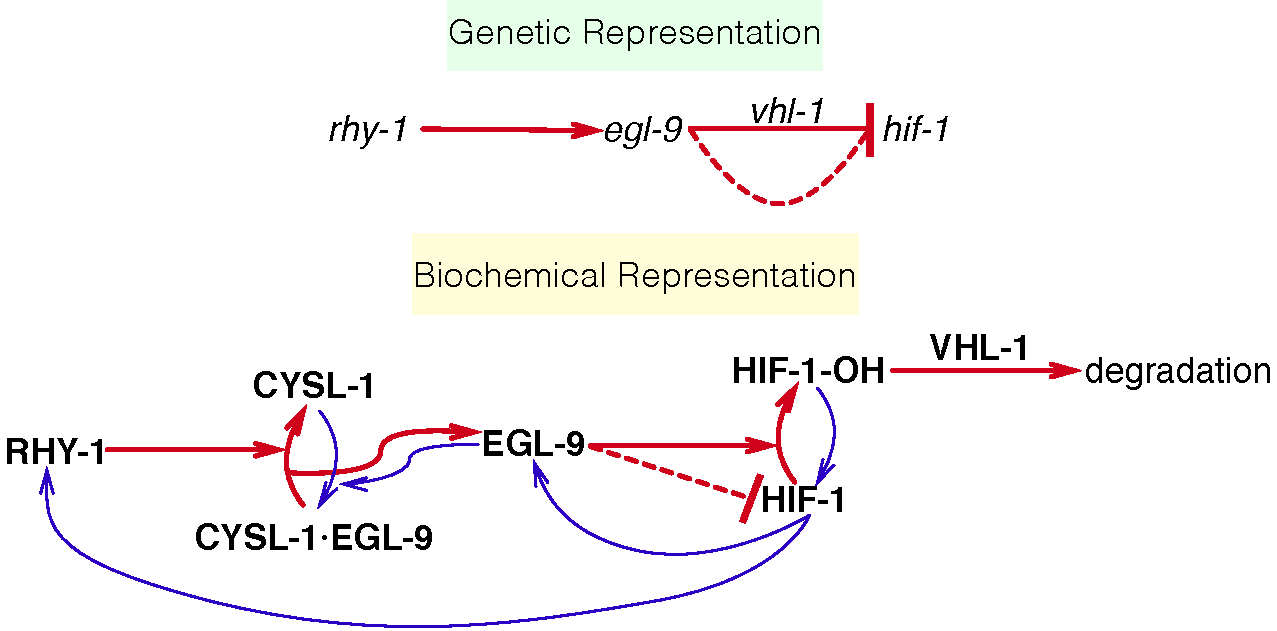
\includegraphics[width=\linewidth]{../figs/HIF1pathway.pdf}
  \caption{
    Genetic and biochemical representation of the hypoxia pathway in \cel{}. Red
    arrows are arrows that lead to inhibition of \hifp{}, and blue arrows are
    arrows that increase \hifp{} activity or are the result of \hifp{} activity.
    \eglp{} is known to exert \vhlp{}-dependent and independent repression
    on \hifp{} as shown in the genetic diagram. The \vhlp{}-independent
    repression of \hifp{} by \eglp{} is denoted by a dashed line and is not
    dependent on the hydroxylating activity of \eglp{}. Technically, RHY-1
    inhibits CYSL-1, which in turn inhibits EGL-9, but this interaction was
    abbreviated in the genetic diagram for clarity.
  }
\label{fig:pathway}
\end{figure}

Our reconstruction of the hypoxia pathway in \cel{} using RNA-sequencing shows
that whole-animal transcriptome profiles can be used as phenotypes genetic
analysis and that the phenomenon of epistasis, a hallmark of genetic
interaction, holds at the molecular systems level. We demonstrate that
transcriptomes can aid in ordering genes in a pathway using only single mutants.
Finally, we were able to identify genes that appear to be downstream of
\gene{egl-9} and \gene{vhl-1}, but do not appear to be targets of \gene{hif-1}.
Using a single set of transcriptome-wide measurements, we observed most of the
known transcriptional effects of \gene{hif-1} as well as novel effects not
described before in \cel{}. Taken together, this demonstrates that whole-animal
RNA-seq is an extremely fast and powerful method for genetic analyses in an area
where phenotypic measurements are now the rate limiting step.


\section*{Results}
\subsection*{The hypoxia pathway controls thousands of genes in \cel{}}
\label{sub:summary}

We selected four single mutants within the hypoxia pathway for expression
profiling: \gene{egl-9}\emph{(sa307)}, \gene{rhy-1}\emph{(ok1402)},
\gene{vhl-1}\emph{(ok161)}, \gene{hif-1}\emph{(ia4)}. We also sequenced the
transcriptomes of two double mutants, \gene{egl-9; vhl-1} and \gene{egl-9 hif-1}
as well as wild-type N2. Each genotype  was sequenced in triplicate at a depth
of 15 million reads per sample. We performed whole-animal RNA-seq at a moderate sequencing
depth ($\sim7$ million mapped reads per sample) under normoxic conditions.
We identified around 22,000 different isoforms per sample, which allowed us to
measure differential expression of 18,344 isoforms across all replicates and
genotypes ($\sim$70\% of the protein coding isoforms in \cel{}). We included in
our analysis a \fog{} (\emph{q71}) mutant we have previously
studied~\cite{Angeles-Albores2016a}, because \gene{fog-2} is not reported to
interact with the hypoxia pathway. We analyzed our data using a general linear
model on logarithm-transformed counts. Changes in gene expression are reflected
in the regression coefficient $\beta$, which is specific to each isoform within
a genotype (excluding wild-type, which is used as baseline). Statistical
significance is achieved when the q-value of a $\beta$ coefficient (p-values
adjusted for multiple testing) are less than 0.1. Genes that are significantly
altered between wild-type and a given mutant (differentially expressed genes,
DEGs) have $\beta$ values that are statistically significantly different from 0
(i.e.\ greater than 0 or less than 0). $\beta$ coefficients are analogous to the
logarithm of the fold-change between mutants and wild-type. Larger magnitudes of
$\beta$ correspond to larger perturbations (see Fig.~\ref{fig:explain}). When we
refer to $\beta$ coefficients and q-values, it will always be in reference to
isoforms. However, we report the sizes of each gene set in by the number of
genes they contain, not isoforms. For the case of \cel{}, this difference is
negligible since the great majority of protein-coding genes have a single
isoform. We have opted for this method of referring to gene sets because it
simplifies the language considerably. A complete version of the code used for
this analysis with ample documentation, is available at
\url{https://wormlabcaltech.github.io/mprsq}.


\begin{figure}[tbhp]
  \centering
  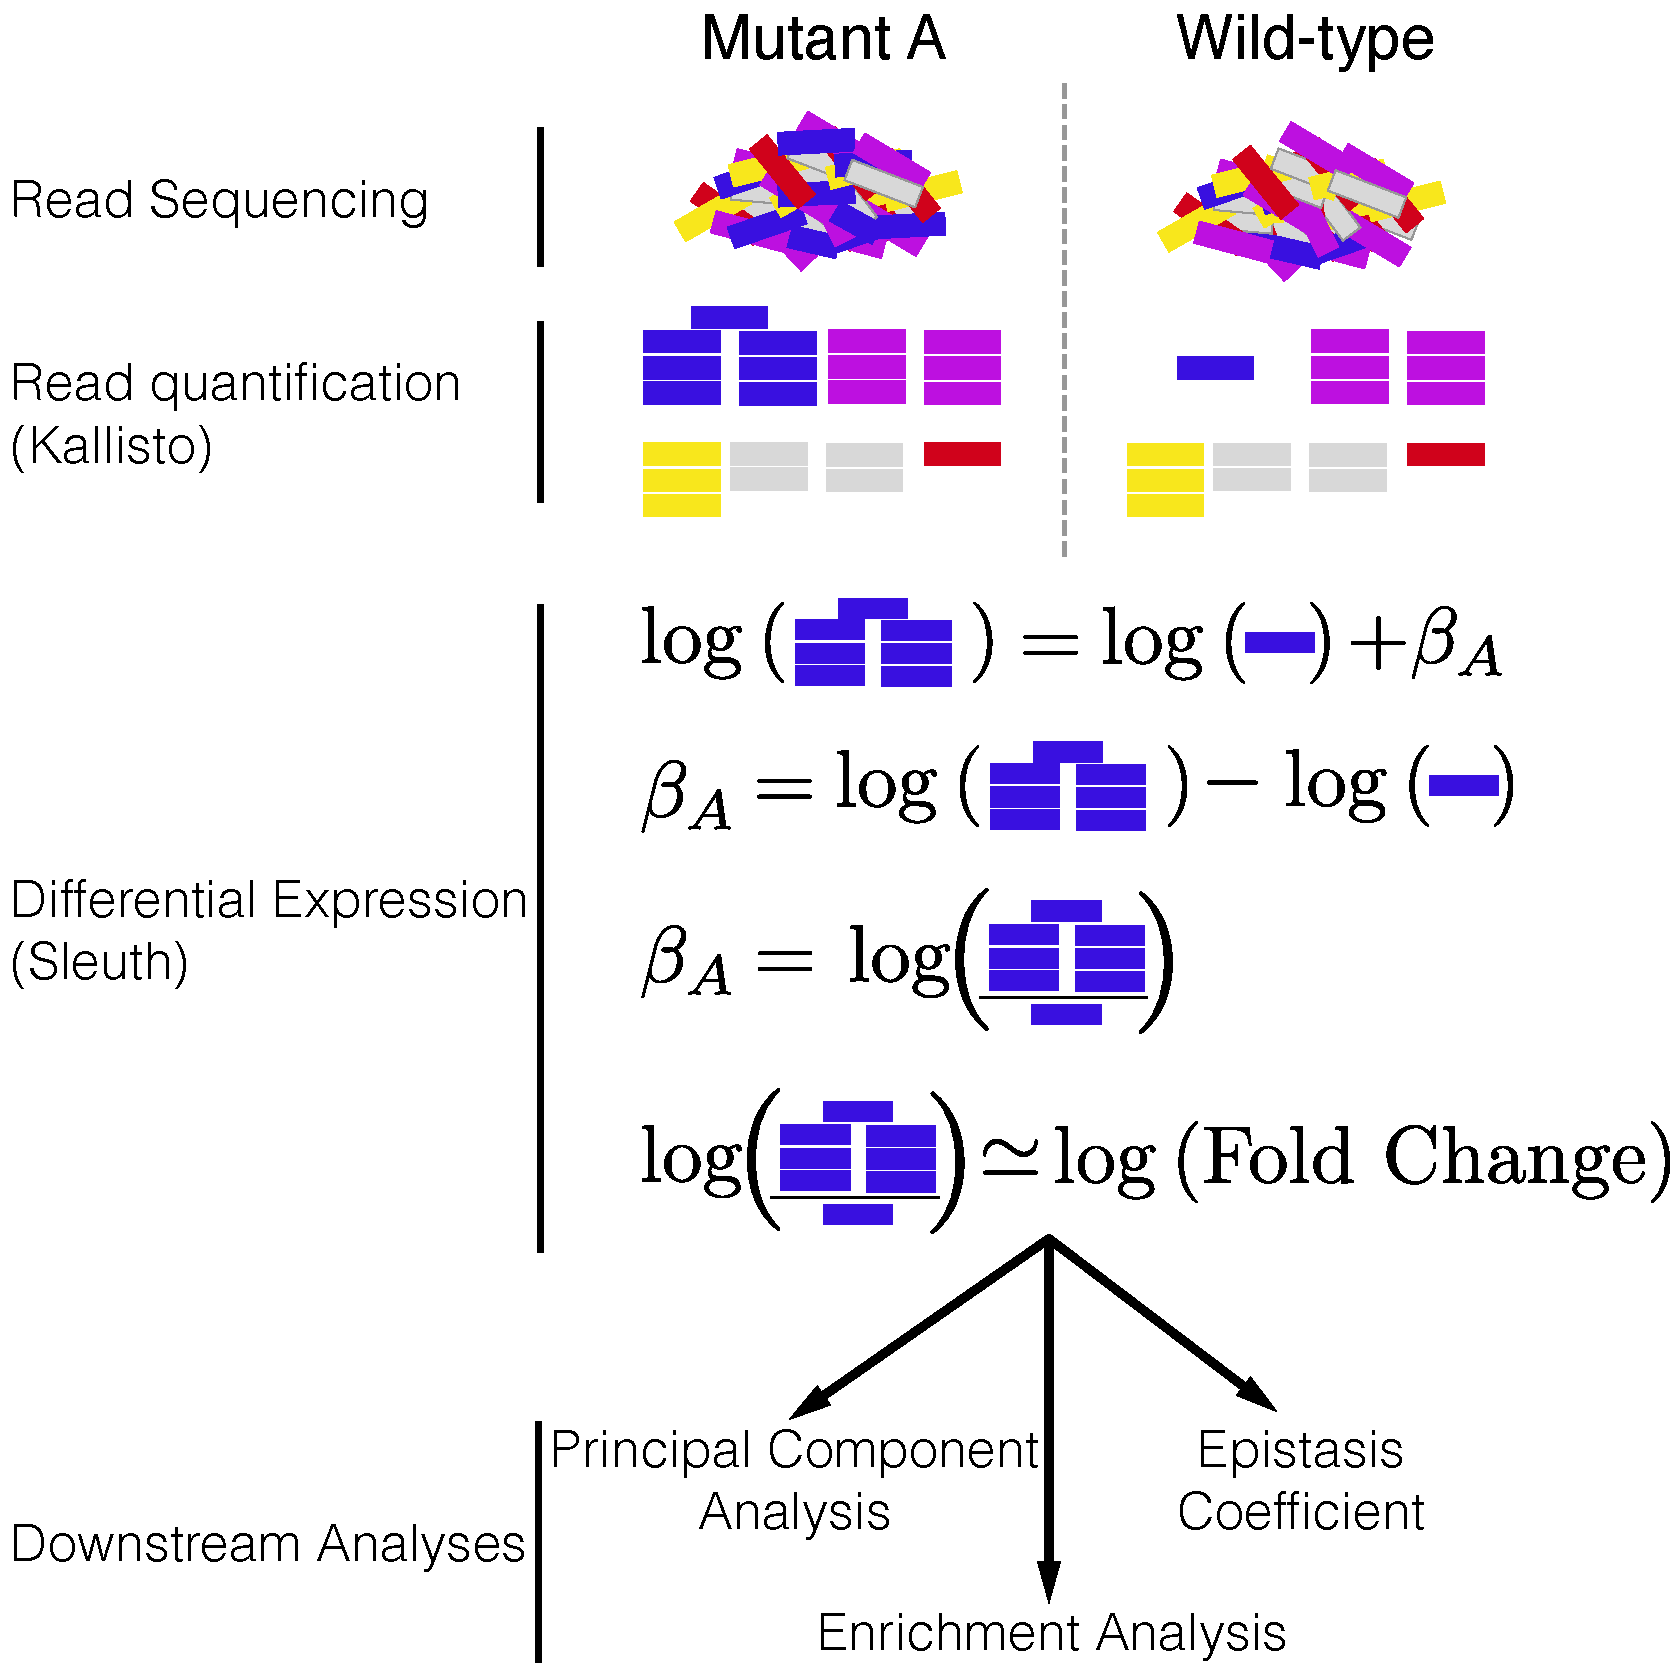
\includegraphics[width=0.35\textwidth]{../figs/meaningofbeta.pdf}
  \caption{
    Analysis workflow. After sequencing, reads are quantified using Kallisto.
    Bars show estimated counts for each isoform. Differential expression is
    calculated using Sleuth, which outputs one $\beta$ coefficient per isoform
    per genotype. $\beta$ coefficients are analogous to the natural logarithm of
    the fold-change relative to a wild-type control. Downstream analyses are
    performed with $\beta$ coefficients that are statistically significantly
    different from 0. Q-values less than 0.1 are considered statistically
    different from 0.
  }
\label{fig:explain}
\end{figure}

Transcriptome profiling of the hypoxia pathway revealed that this pathway
controls thousands of genes in \cel{}. The \egl{} transcriptome showed
differential expression of \egln{} genes. Similarly, \rhyn{} genes were
differentially expressed in \rhy{} mutants. The \vhl{} transcriptome showed
considerably fewer DEGs (\vhln{}), possibly because it
is a weaker inhibitor of \hif{} than \egl{}~\cite{Shao2009}. The \egl{};\vhl{}
double mutant transcriptome showed \eglvhln{} DEGs.
The \hif{} mutant also showed a transcriptomic phenotype involving \hifn{}
genes. The \eglhif{} double mutant showed a similar number of genes with altered
expression (\eglhifn{} genes, Table~\ref{tab:genes}).


\begin{table}[tbhp]
  \centering
  \begin{tabular}{lr}
    \toprule{}
    Genotype & Differentially Expressed Genes\\
    \midrule{}\egl{} & \egln{}\\
    \rhy{} & \rhyn{}\\
    \vhl{} & \vhln{}\\
    \hif{} & \hifn{}\\
    \eglvhl{} & \eglvhln{}\\
    \eglhif{} & \eglhifn{}\\
    \fog{} & \fogn{}\\
    \bottomrule{}
  \end{tabular}
  \caption{Number of differentially expressed genes in each mutant with respect
  to wild-type (N2).}
\label{tab:genes}
\end{table}

\subsection*{Principal Component Analysis visualizes epistatic relationships
             between genotypes}
\label{sub:Clustering}

PCA is used to identify relationships between high-dimensional data
points~\cite{Yeung2001}. We performed PCA on our data to examine whether each
genotype clustered in a biologically relevant manner. PCA identifies the vector
that can explain most of the variation in the data; this is called the first PCA
dimension. Using PCA, one can identify the first $n$ dimensions that can explain
more than 95\% of the variation in the data. Sample clustering in these $n$
dimensions often indicates biological relationships between the data, although
interpreting PCA dimensions can be difficult.

% After applying PCA, we expected \hif{} to cluster near \eglhif{}, because
% \hif{} exhibits no phenotypic defects under normoxic conditions, in contrast to
% \egl{}, which exhibits an egg-laying (Egl) phenotype in the same environment.
% In \eglhif{} mutants the Egl phenotype of \egl{} mutants is suppressed and instead
% the grossly wild-type phenotype of \hif{} is observed. On the other hand, we
% expected \egl{}, \rhy{}, \vhl{} and \eglvhl{} to form a separate cluster since
% each of these genotypes is Egl and has a constitutive hypoxic response. Finally,
% we included as a negative control a \fog{} mutant we have analyzed
% previously~\cite{Angeles-Albores2016a}. This data was obtained at a different
% time from the other genotypes, so we included a batch-normalization term in our
% equations to account for this. Since \gene{fog-2} has not been described
% to interact with the hypoxia pathway, we expected that it should appear far away
% from either cluster.

The first dimension of the PCA analysis was able to discriminate between mutants
that have constitutive high levels of \hifp{} and mutants that have no \hifp{},
whereas the second dimension was able to discriminate between mutants within the
hypoxia pathway and outside the hypoxia pathway (see Fig.~\ref{fig:pca};
\gene{fog-2} is not reported to act in the hypoxia pathway and acts as a
negative control). Therefore, expression profiling measures enough signal to
cluster genes in a meaningful manner in complex metazoans.

\begin{figure}[tbhp]
  \centering
  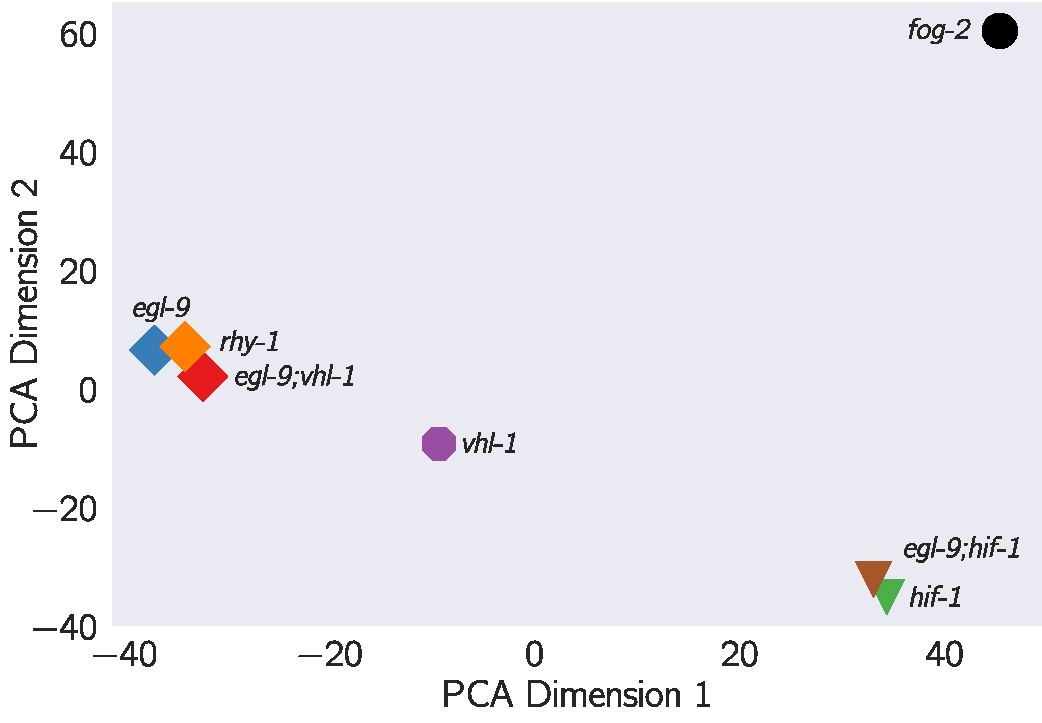
\includegraphics[width=0.4\textwidth]{../figs/pca.pdf}
  \caption{
    Principal component analysis of various \cel{} mutants. Genotypes that have
    an constitutive hypoxia response (i.e. \egl{}) cluster far from genotypes
    that do not have a hypoxic response (i.e. \hif{}) along PCA Dimension 1. PCA
    Dimension 2 separates genotypes that do not participate hypoxic response
    pathway.
  }
\label{fig:pca}
\end{figure}

\subsection*{Reconstruction of the hypoxia pathway from first genetic principles}
\label{sec:reconstruct}
To reconstruct a genetic pathway, we must first assess whether two genes act on
the same phenotype. If they do not act on the same phenotype (two mutations do
not cause the same genes to become differentially expressed relative to
wild-type), these mutants are independent. Otherwise, we must measure whether
these genes act additively or epistatically on the phenotype of interest; if
there is epistasis we must measure whether it is positive or negative, in order
to assess whether the epistatic relationship is a genetic suppression or a
synthetic interaction. To allow coherent comparisons of different mutant
transcriptomes (the phenotype we are studying here), we define the shared
transcriptomic phenotype between two mutants (STP) as the shared set of genes or
isoforms whose expression in both mutants are different from that in wild-type,
regardless of the direction of change

\subsubsection*{Genes in the hypoxia mutant act on the same transcriptional
                phenotype}
\label{sec:phenotypes}
All the hypoxia mutants had a significant STP:\@ the fraction of differentially
expressed genes that was shared between mutants ranged from a minimum of 10\%
shared between \hif{} and \eglvhl{} to a maximum of 32\% shared genes between
\egl{} and \eglvhl{}. For comparison, we also analyzed a previously published
\fog{} transcriptome~\cite{Angeles-Albores2016a}. The \gene{fog-2} gene is
involved in masculinization of the \cel{} germline, which enables sperm
formation, and is not known to be involved in the hypoxia pathway. The hypoxia
pathway mutants and the \fog{} mutant also showed shared transcriptomic
phenotypes (8.8\%--14\% genes).

% genetic correlations
\begin{figure}[tbhp]
  \centering
  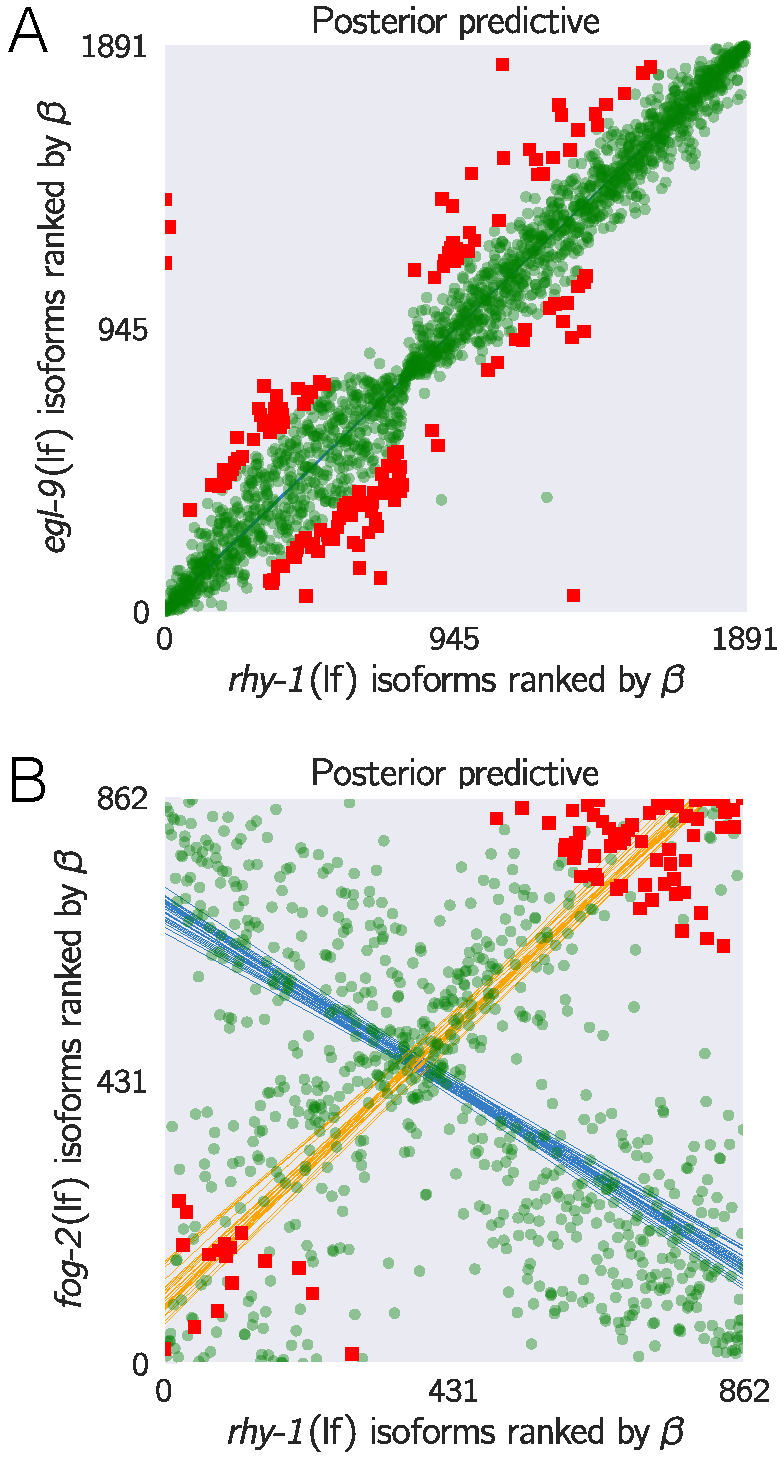
\includegraphics[width=.4\textwidth]{../figs/positive_and_control.pdf}
  \caption{
    Strong transcriptional correlations can be identified between genes that
    share a positive regulatory connection.
    \textbf{A}. We obtained identified
    isoforms that were differentially expressed in both \egl{} and the \rhy{}
    mutants, and ranked each isoform according to its $\beta$ coefficient. We
    plotted the rank of each gene in \rhy{} versus the rank of the same gene in
    the \egl{} transcriptome.
    \textbf{B}. For comparison, we followed the same
    procedure with the \fog{} and \rhy{} transcriptomes. \fog{} is not known to
    interact with the primary hypoxia pathway.
    Green, transparent large points
    mark inliers to the primary regressions (blue lines); red squares mark
    outliers to the primary regressions and orange lines represent the secondary
    correlations involving the outliers.
  }
\label{fig:genetic_interactions}
\end{figure}

Next, we performed pairwise correlations between all mutant pairs. We
rank-transformed the $\beta$ coefficients of each isoform between the STP of two
mutants, and calculated lines of best fit using Bayesian regressions that are
robust to outliers (see Fig~\ref{fig:genetic_interactions}). For mutants
associated with the hypoxia pathway, these correlations have values higher than
0.9 with a tight distribution around the line of best fit. The correlations for
mutants from the hypoxia pathway with the \fog{} mutant were considerably
weaker, with magnitudes between 0.6--0.85 and greater variance around the line
of best fit. Although \gene{hif-1} is known to be genetically repressed by
\gene{egl-9}, \gene{rhy-1} and \gene{vhl-1}~\cite{Epstein2001,Shen2006}, all the
correlations between mutants of these genes and \hif{} were positive.


\subsection*{Transcriptome-wide epistasis}
Ideally, any measurement of transcriptome-wide epistasis should conform to
certain expectations. First, it should make use of the regression coefficients
of as many genes as possible. Second, it should be summarizable in a single,
well-defined number. Third, it should have an intuitive behavior, such that
special values of the statistic have an unambiguous interpretation.

We discovered a method that satisfies all of the above condition and which can
be graphed in a plot we call an epistasis plot (see Fig~\ref{fig:egl9epistasis})
In an epistasis plot, the X-axis represents the expected expression of a double
mutant $a^-b^-$ if $a$ and $b$ interact log-additively. In other words, each
individual isoform's x-coordinate is the sum of the regression coefficients from
the single mutants $a^-$ and $b^-$. The Y-axis represents the deviations from
the log-additive (null) model, and can be calculated as the difference between
the observed regression coefficient and the predicted regression coefficient.
Only genes that are differentially expressed in all three genotypes are plotted.
These plots will generate specific patterns that can be described through linear
regressions. The slope of these lines, $s_{a,b}$, is the transcriptome-wide
epistasis coefficient.

Transcriptome-wide epistasis coefficients can be understood intuitively for
simple cases of genetic interactions if true genetic nulls are used. If two
genes act additively on the same set of differentially expressed isoforms then
all the plotted points will fall along the line $y=0$. If two genes act
positively in an unbranched pathway, then all the mutants should have the same
phenotype. It follows that data from this pathway will form line with slope
equal to $-\frac{1}{2}$. On the other hand, in the limit of complete inhibition
of $a$ by $b$ in an unbranched pathway, the plots should show a line of best fit
with slope equal to $-1$.
Genes that interact synthetically (\emph{i.e.}, through an OR-gate)
will fall along lines with slopes $>0$. When there is epistasis of one gene over
another, the points will fall along a line with slope $s_{ab=b}$ or $s_{ab=a}$.
We can use the single mutant data to predict the distribution of slopes that
results for each case stated above. The transcriptome-wide epistasis coefficient
emerges as a powerful way to quantify epistasis because it integrates
information from many different isoforms into a single number (see
Fig.~\ref{fig:egl9epistasis}).

In our experiment, we studied two double mutants, \eglhif{} and \eglvhl{}. We
wanted to understand how well an epistatic analysis based on transcriptome-wide
coefficients agreed with the epistasis results reported in the literature, which
were based on qPCR of single genes. Therefore, we performed orthogonal distance
regression on the two gene combinations we studied (\gene{egl-9} and
\gene{vhl-1}; and \gene{egl-9} and \gene{hif-1}) to determine the epistasis
coefficient for each gene pair. We also generated models for the special cases
mentioned above using the single mutant data.


We measured the epistasis coefficient between \gene{egl-9} and \gene{vhl-1} and
$s_{\text{\gene{egl-9} \gene{vhl-1}}} = -0.41$. Simulations using just the
single mutant data showed that the double mutant behaved exactly as expected (in
other words, \egl{} = \eglvhl{}, see Fig.~\ref{fig:egl9epistasis}). We used
Bayesian model selection to reject a linear pathway ($OR>10^{83}$). We also
measured epistasis between \gene{egl-9} and \gene{hif-1},
$s_{\text{\gene{egl-9}, \gene{hif-1}}} = -0.80$. This is consistent with a
pathway where \gene{hif-1} is inhibited by \gene{egl-9} (\hif{} =
\eglhif{}) and we reject the null hypothesis that these two genes act in a
positive linear pathway ($OR > 10^{93}$).

% epistasis graph
\begin{figure}[tbhp]
  \centering
  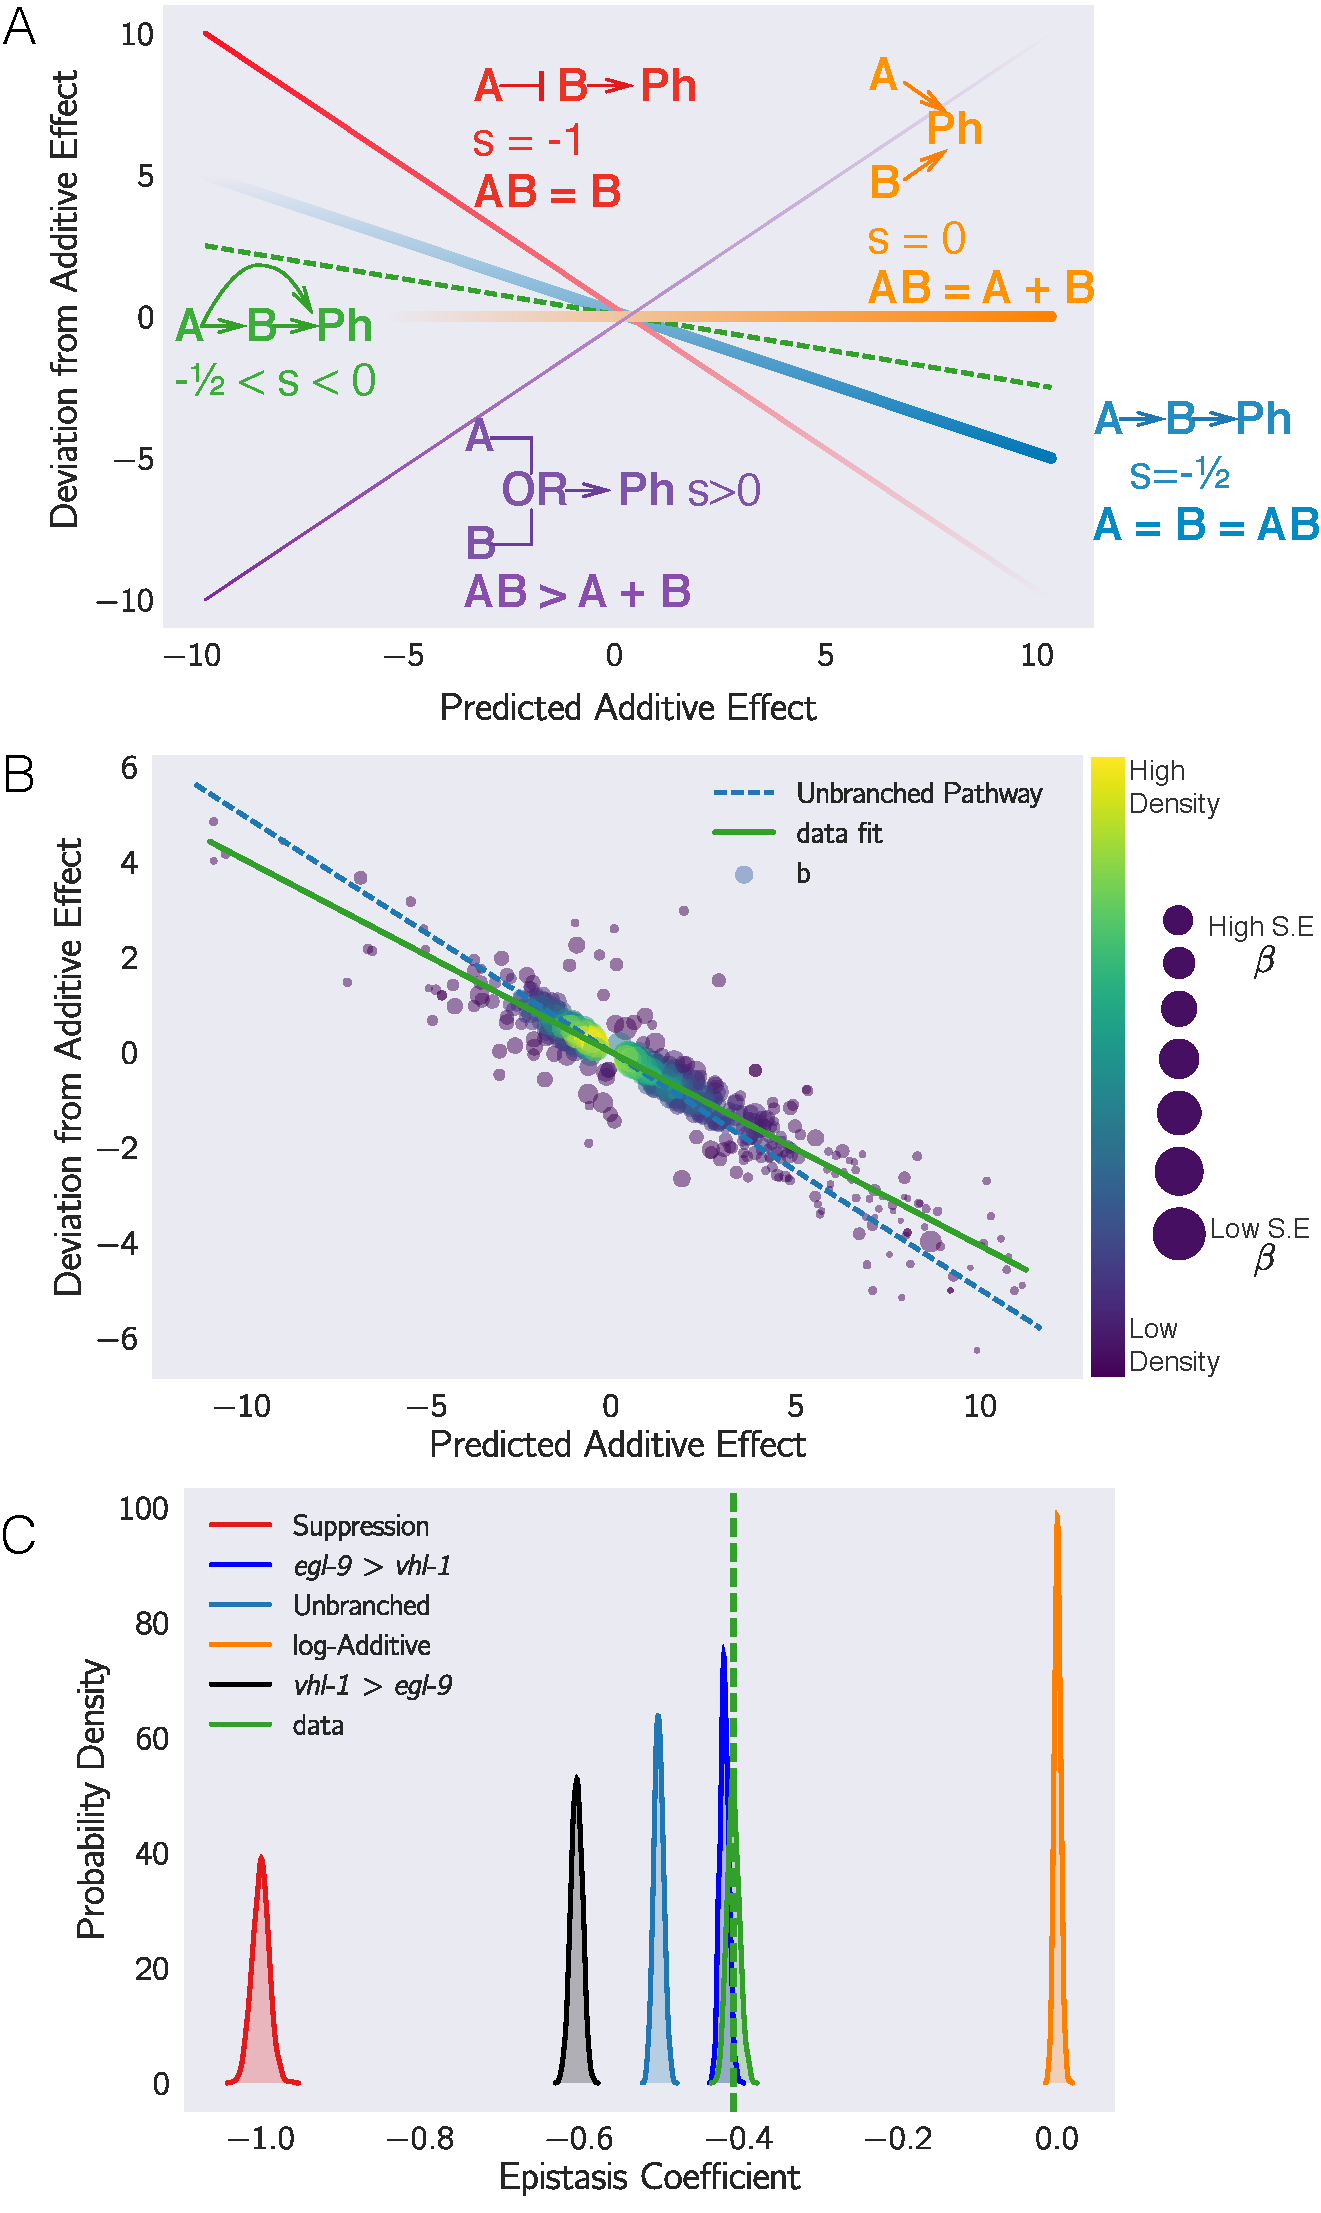
\includegraphics[width=0.5\textwidth]{../figs/egl9vhl1-epistasis.pdf}
  \caption{
    (\textbf{A}) Schematic diagram of an epistasis plot. The X-axis on an
    epistasis plot is the expected coefficient for a double mutant under an
    log-additive model (null model). The Y-axis plots deviations from this
    model. Double mutants that deviate in a systematic manner from the null
    model exhibit transcriptome-wide epistasis ($s$). To measure $s$, we find
    the line of best fit and determine its slope. Genes that act log-additively
    on a phenotype \textbf{(Ph)} will have $s=0$ (null hypothesis, orange line);
    whereas genes that act along an unbranched pathway will have $s=-1/2$ (blue
    line). Strong repression is reflected by $s=-1$ (red line), whereas $s>0$
    correspond to synthetic interactions (purple line). (\textbf{B}) Epistasis
    plot showing that the \eglvhl{} transcriptome deviates significantly from a
    null additive. Points are colored qualitatively according to density
    (purple---low, yellow---high) and size is inversely proportional to the
    standard error (S.E.) of the y-axis. The green line is the line of best fit
    from an orthogonal distance regression. (\textbf{C}) Comparison of simulated
    epistatic coefficients against the observed coefficient. Green curve shows
    the bootstrapped observed transcriptome-wide epistasis coefficient for
    \gene{egl-9} and \gene{vhl-1}. Dashed green line shows the mean value of the
    data. Simulations use only the single mutant data to idealize what
    expression of the double mutant should look like. $x > y$ means that the
    phenotype of $x$ is observed in a double mutant $x^-y^-$. }
\label{fig:egl9epistasis}
\end{figure}

\subsubsection*{Epistasis can be predicted}
Given our success in measuring epistasis coefficients, we wanted to know whether
we could predict the epistasis coefficient between \gene{egl-9} and \gene{vhl-1}
in the absence of the \egl{} genotype. Since \rhyp{} indirectly activates
\eglp{}, the \rhy{} transcriptome should contain more or less equivalent
information to the \egl{} transcriptome. Therefore, we generated predictions of
the epistasis coefficient between \gene{egl-9} and \gene{vhl-1} by substituting
in the \rhy{} data. We predicted $s_{rhy-1,vhl-1} = -0.45$. Similarly, we used
the \eglvhl{} double mutant to measure the epistasis coefficient while replacing
the \egl{} dataset with the \rhy{} dataset. We found that the epistasis
coefficient using this substitution was $-0.40$. This coefficient was different
from $-0.50$ (OR $>10^{62}$), reflecting the same qualitative conclusion that
the hypoxia pathway is branched. In conclusion, we were able to obtain a
quantitatively close prediction of the epistasis coefficient for two mutants
using the transcriptome of a related, upstream mutant. Finally, in the absence
of a single mutant, an upstream locus can be used to estimate epistasis between
two genes.

\subsection*{Transcriptomic decorrelation can be used to infer functional distance}
\label{sub:decorrelation}
% What are functional interactions?
So far, we have shown that RNA-seq can accurately measure genetic interactions.
However, genetic interactions do not require two gene products to interact
biochemically, nor even to be physically close to each other. RNA-seq cannot
measure physical interactions between genes, but we wondered whether expression
profiling contains sufficient information to order genes along a pathway.

Single genes are often regulated by multiple independent sources. The connection
between two nodes can in theory be characterized by the strength of the edges
connecting them (the thickness of the edge); the sources that regulate both
nodes (the fraction of inputs common to both nodes); and the genes that are
regulated by both nodes (the fraction of outputs that are common to both nodes).
In other words, we expected that expression profiles associated with a pathway
would respond quantitatively to quantitative changes in activity of the pathway.
Targeting a pathway at multiple points would lead to expression profile
divergence as we compare nodes that are separated by more degrees of freedom,
reflecting the flux in information between them.

% decorrelation
\begin{figure}[tbhp]
  \centering
  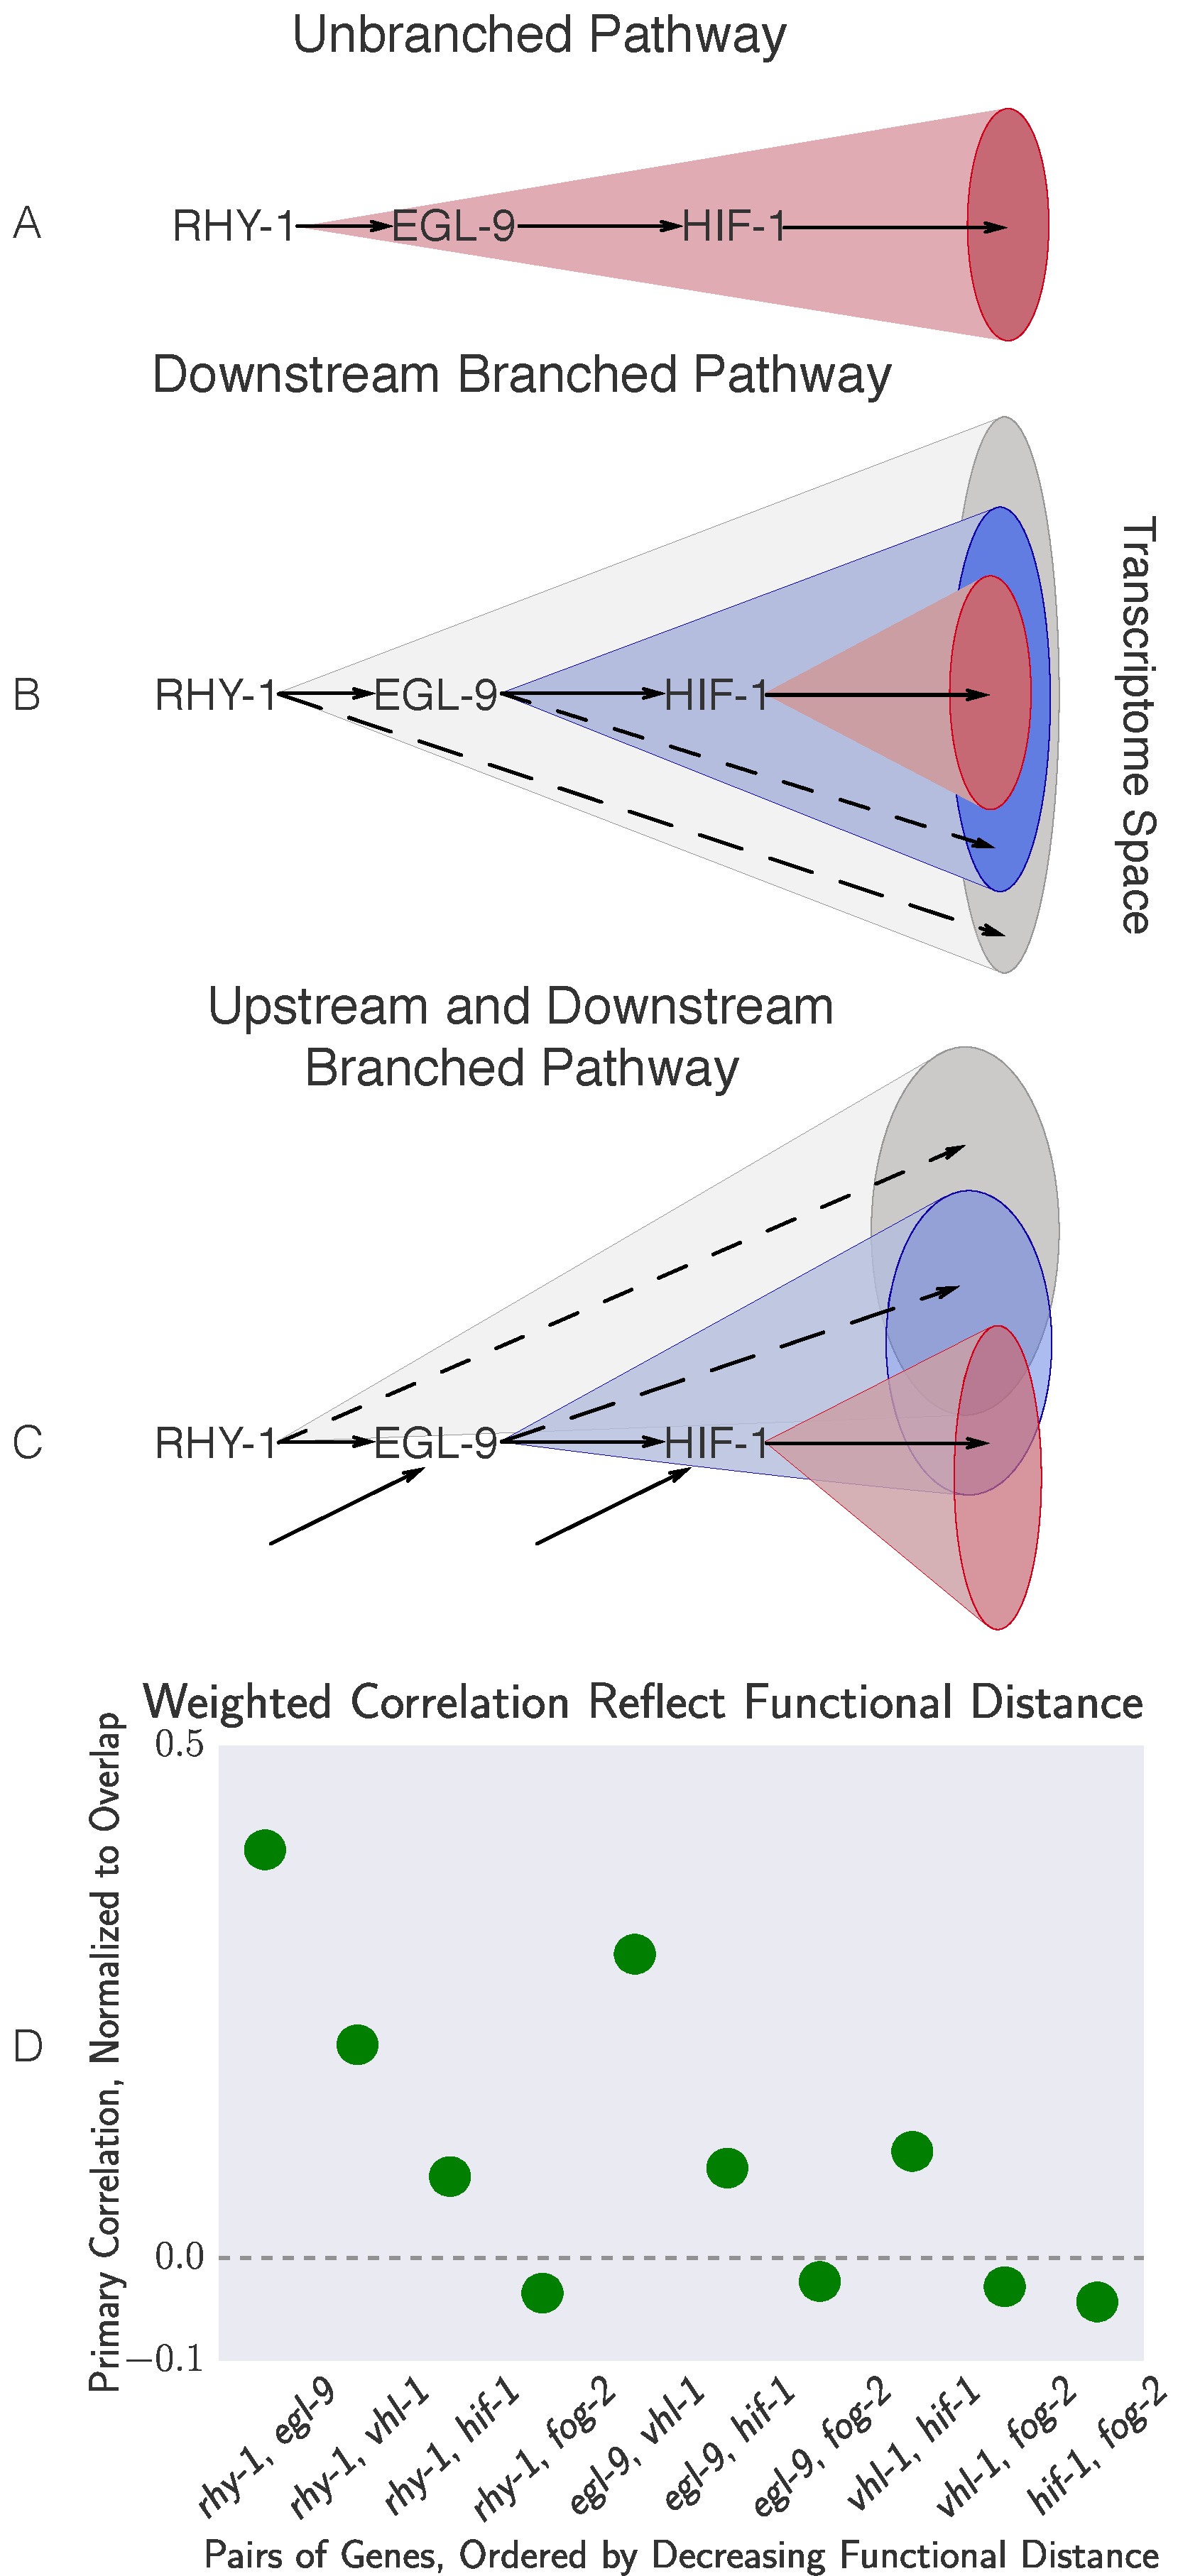
\includegraphics[width=.4\textwidth]{../figs/decorrelation.pdf}
  \caption{
    Theoretically, transcriptomes can be used to order genes in a pathway under
    certain assumptions. Arrows in the diagrams above are intended to show the
    direction of flow, and do not indicate valence. \textbf{A}. A linear pathway
    in which \gene{rhy-1} is the only gene controlling \gene{egl-9}, which in
    turn controls \gene{hif-1} does not contain information to infer the order
    between genes. \textbf{B}. If \gene{rhy-1} and \gene{egl-9} have
    transcriptomic effects that are separable from \gene{hif-1}, then the
    \gene{rhy-1} transcriptome should contain contributions from \gene{egl-9},
    \gene{hif-1} and \gene{egl-9}- and \gene{hif-1}-independent pathways. This
    pathway contains enough information to infer order. \textbf{C}. If a pathway
    is branched both upstream and downstream, transcriptomes will show even
    faster decorrelation. Nodes that are separated by many edges may begin to
    behave almost independently of each other with marginal transcriptomic
    overlap or correlation. \textbf{D}. The hypoxia pathway can be ordered. We
    hypothesize the rapid decay in correlation is due to a mixture of upstream
    and downstream branching that happens along this pathway. Bars show the
    standard error of the weighted coefficient from the Monte Carlo Markov Chain
    computations.
  }
\label{fig:decorrelation}
\end{figure}

We investigated this possibility by weighting the robust Bayesian regression
between each pair of genotypes by the size of the shared transcriptomic
phenotype of each pair divided by the total number of isoforms differentially
expressed in either mutant ($N_\mathrm{Intersection}/N_{\mathrm{Union}}$). We
plotted the weighted correlation of each gene pair, ordered by increasing
functional distance (see Fig.~\ref{fig:decorrelation}). In every case, we see
that the weighted correlation decreases monotonically due mainly, but not
exclusively, to a smaller STP.\@We believe that this result is not due to random
noise or insufficiently deep sequencing. Instead, we propose a framework in
which every gene is regulated by multiple different molecular species, which
induces progressive decorrelation. This decorrelation in turn has two
consequences. First, decorrelation within a pathway implies that two nodes may
be almost independent of each other if the functional distance between them is
large. Second, it may be possible to use decorrelation dynamics to infer gene
order in a branching pathway, as we have done with the hypoxia pathway.

\subsection*{The circuit topology of the hypoxia pathway explains patterns in
            the data}
\label{sub:topology}
While some of the rank plots contained a clear positive
correlation (see Fig.~\ref{fig:genetic_interactions}), others showed a
discernible cross-pattern (see Fig.~\ref{fig:xpattern}). In particular, this
cross-pattern emerged between \vhl{} and \rhy{} or between \vhl{} and \egl{},
even though \gene{vhl-1}, \gene{rhy-1} and \gene{egl-9} are all
inhibitors of \hif{}. Such cross-patterns could be indicative of feedback loops
or other complex interaction patterns.
If the above is correct, then it should be possible to identify genes that are
regulated by \gene{rhy-1} in a logically consistent way: Since loss of
\gene{egl-9} causes \gene{rhy-1} mRNA levels to increase, if this increase leads
to a significant change in RHY-1 activity, then it follows that the \egl{} and
\rhy{} should show anti-correlation in a subset of genes.
Since we do not observe many genes that are anti-correlated, we conclude that is
unlikely that the change in \gene{rhy-1} mRNA expression causes a significant
change in RHY-1 activity under normoxic conditions.

We identified a main hypoxia response induced by HIF-1 (655 genes) by
identifying genes that were consistently upregulated in \egl{}, \rhy{} and
\vhl{} mutants. This response included five transcription factors
(\gene{W02D7.6}, \nhr{}, \gene{ztf-18}, \gene{nhr-135} and \gene{dmd-9};
Supplementary Table 1).

\gene{hif-1}-independent effects of \gene{egl-9} have been reported
previously~\cite{Park2012}, which led us to question whether we could identify
similar effects in our dataset. We have observed that \hif{} displays a modest
increase in the transcription of \gene{rhy-1}, from which we speculated that
\eglp{} would have increased activity in the \hif{} mutant compared to the
wild-type. Therefore, we searched for genes that were regulated in an opposite
manner between \hif{} and \eglhif{}, and that were regulated in the same
direction between all \egl{} genotypes.

We also searched for genes with \gene{hif-1}-independent, \gene{vhl-1}-dependent
gene expression and found \vhltargets{} genes (Supplementary Table 2). Finally,
we searched for candidates directly regulated by \gene{hif-1}. Initially, we
searched for genes that were significantly altered in \hif{} genotypes in one
direction, but altered in the opposite direction in mutants that activate the
\hifp{} response. Only five genes (\gene{R08E5.3}, \gene{cysl-2}, \gene{nit-1},
\gene{sqrd-1} and \gene{hsp-12.3}) met these conditions. We reasoned that genes
that are overexpressed in mutants that induce the \hifp{} response would be
enriched for genes that are directly regulated by \hifp{}. We found
\hiftargets{} such genes (Supplementary Table 3).

\subsection*{Identification of non-classical epistatic interactions}
\label{sub:hifoh}
\hif{} has traditionally been viewed as existing in a genetic OFF state under
normoxic conditions. However, our dataset indicates that \hifn{} genes show
altered expression when \gene{hif-1} function is removed in normoxic conditions.
Moreover, we observed positive correlations between \hif{} $\beta$ coefficients
and \egl{}, \vhl{} and \rhy{} $\beta$ coefficients in spite of the negative
regulatory relationships between these genes and \gene{hif-1}. Such positive
correlations could indicate a relationship between these genes that has not
been reported previously.

We first identified genes that exhibited violations of the canonical genetic
model of the hypoxia pathway. We searched for genes that changed in different
directions between \egl{} and \vhl{}, or, equivalently, between \rhy{} and
\vhl{} (we assume that all results from the \rhy{} transcriptome reflect a
complete loss of \gene{egl-9} activity). We found \hifohtargets{} that satisfied
this condition (see Fig.~\ref{fig:hif1oh}, Supplemental Table 4). Regardless of
this behavior, \gene{egl-9} remained epistatic over \gene{vhl-1} for this class
of genes.

\begin{figure}[tbhp]
  \centering
  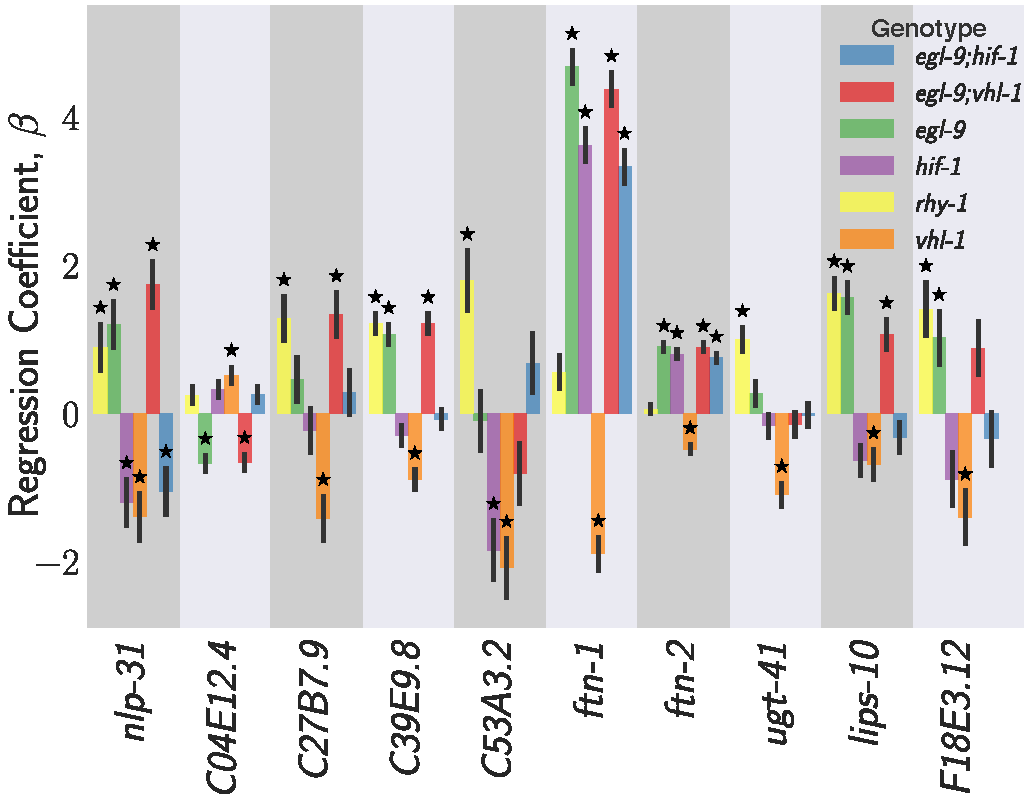
\includegraphics[width=.4\textwidth]{../figs/hif1oh_epistasis.pdf}
  \caption{
    \textbf{A}. \hifohtargets{} genes in \cel{} exhibit non-classical epistasis
    in the hypoxiapathway, characterized by opposite effects on gene expression,
    relative to the wild-type, of of the \vhl{} compared to \egl{} (or \rhy{})
    mutants. Shown are a random selection of 15 out of \hifohtargets{} genes for
    illustrative purposes. \textbf{B}. Genes that behave non-canonically  have a
    consistent pattern. \vhl{} mutants have an opposite effect to \egl{}, but
    \gene{egl-9} remains epistatic to \gene{vhl-1} and loss-of-function
    mutations in \gene{hif-1} suppress the \egl{} phenotype. Asterisks show
    $\beta$ values significantly different from 0 relative to wild-type
    (\qval{1}).
  }
\label{fig:hif1oh}
\end{figure}

Although this entire class had similar behavior, for simplicity we focused on
two genes, \nlp{} and\ftna{} which have expression patterns representative
of this class. \ftna{} and \ftnb{} are both described in
the literature as genes that are responsive to mutations in the hypoxia pathway.
These genes have been previously described to have aberrant
behaviors~\cite{Ackerman2012,Romney2011}; specifically, the opposite effects of
\egl{} and \vhl{}. These studies showed the same patterns of \ftna{}
expression phenotypes using both RNAi and alleles, which allays concerns of
strain-specific interference.
We observed that \gene{hif-1} was epistatic to
\gene{egl-9}, and that \gene{egl-9} and \gene{hif-1} both promoted \ftna{} and
\ftnb{} expression.

Analysis of \ftna{} expression reveals that \gene{egl-9} is
epistatic to \gene{hif-1}; that \gene{vhl-1} has opposite effects to
\gene{egl-9}, and that \gene{vhl-1} is epistatic to \gene{egl-9}. Analysis of
\nlp{} reveals similar relationships. \nlp{} expression is decreased in \hif{},
and increased in \egl{}. However, \gene{egl-9} is epistatic to \gene{hif-1}.
Like \ftna{} \gene{vhl-1} has the opposite effect to \gene{egl-9},
yet is epistatic to \gene{egl-9}. We propose in the Discussion a model for how
\hifp{} might regulate these targets.


\section*{Discussion}
\label{sec:discussion}
\subsection*{The \cel{} hypoxia pathway can be reconstructed entirely from
             RNA-seq data}
In this paper, we have shown that whole-organism transcriptomic phenotypes
can be used to reconstruct genetic pathways and to discern previously overlooked
or uncharacterized genetic interactions. We successfully reconstructed the hypoxia
pathway, and inferred order of action (\gene{rhy-1} activates \gene{egl-9},
\gene{egl-9} and \gene{vhl-1} inhibit \gene{hif-1}), and we were able to infer
from transcriptome-wide epistasis measurements that \gene{egl-9} exerts
\gene{vhl-1}-dependent and independent inhibition on \gene{hif-1}.

\subsection*{Interpretation of the non-classical epistasis in the hypoxia pathway}
The observation of \hifohtargets{} genes that exhibit a specific pattern of
non-classical epistasis suggests the existence of previously undescribed aspects
of the hypoxia pathway. Some of these non-classical behaviors had been observed
previously~\cite{Ackerman2012,Romney2011,Luhachack2012}, but no satisfactory
mechanism has been proposed to explain this biology. Previous
studies~\cite{Romney2011,Ackerman2012} suggest that \hifp{} integrates
information on iron concentration in the cell to bind to the \ftna{} promoter,
but could not definitively establish a mechanism. It is unclear why deletion of
\gene{hif-1} and deletion of \gene{egl-9} both cause induction of \ftna{}
expression, but deletion of \gene{vhl-1} abolishes this induction. Moreover,
Luchachack et al~\cite{Luhachack2012} have previously reported that certain
genes important for the \cel{} immune response against pathogens reflect similar
non-canonical expression patterns. Their interpretation was that \gene{swan-1},
which encodes a binding partner to \eglp{}~\cite{Shao2010}, is important for
modulating \hifp{} activity in some manner. The lack of a conclusive double
mutant analysis in this work means the role of SWAN-1 in modulation of \hifp{}
activity remains to be demonstrated. Other mechanisms, such as tissue-specific
differences in the pathway~\cite{Budde2010} could also modulate expression,
though it is worth pointing out that \ftna{} expression appears restricted to a
single tissue, the intestine~\cite{Kim2004}. Another possibility is that
\gene{egl-9} controls \gene{hif-1} mRNA stability via other
\gene{vhl-1}-independent pathways, but we did not decreases in \gene{hif-1}
level in \egl{}, \rhy{} or \vhl{} mutants. Another possibility, such as control
of protein stability via \gene{egl-9} independently of
\gene{vhl-1}~\cite{Chintala2012} will not lead to splitting unless it happens in
a tissue-specific manner.

\begin{figure}[tbhp]
  \centering
  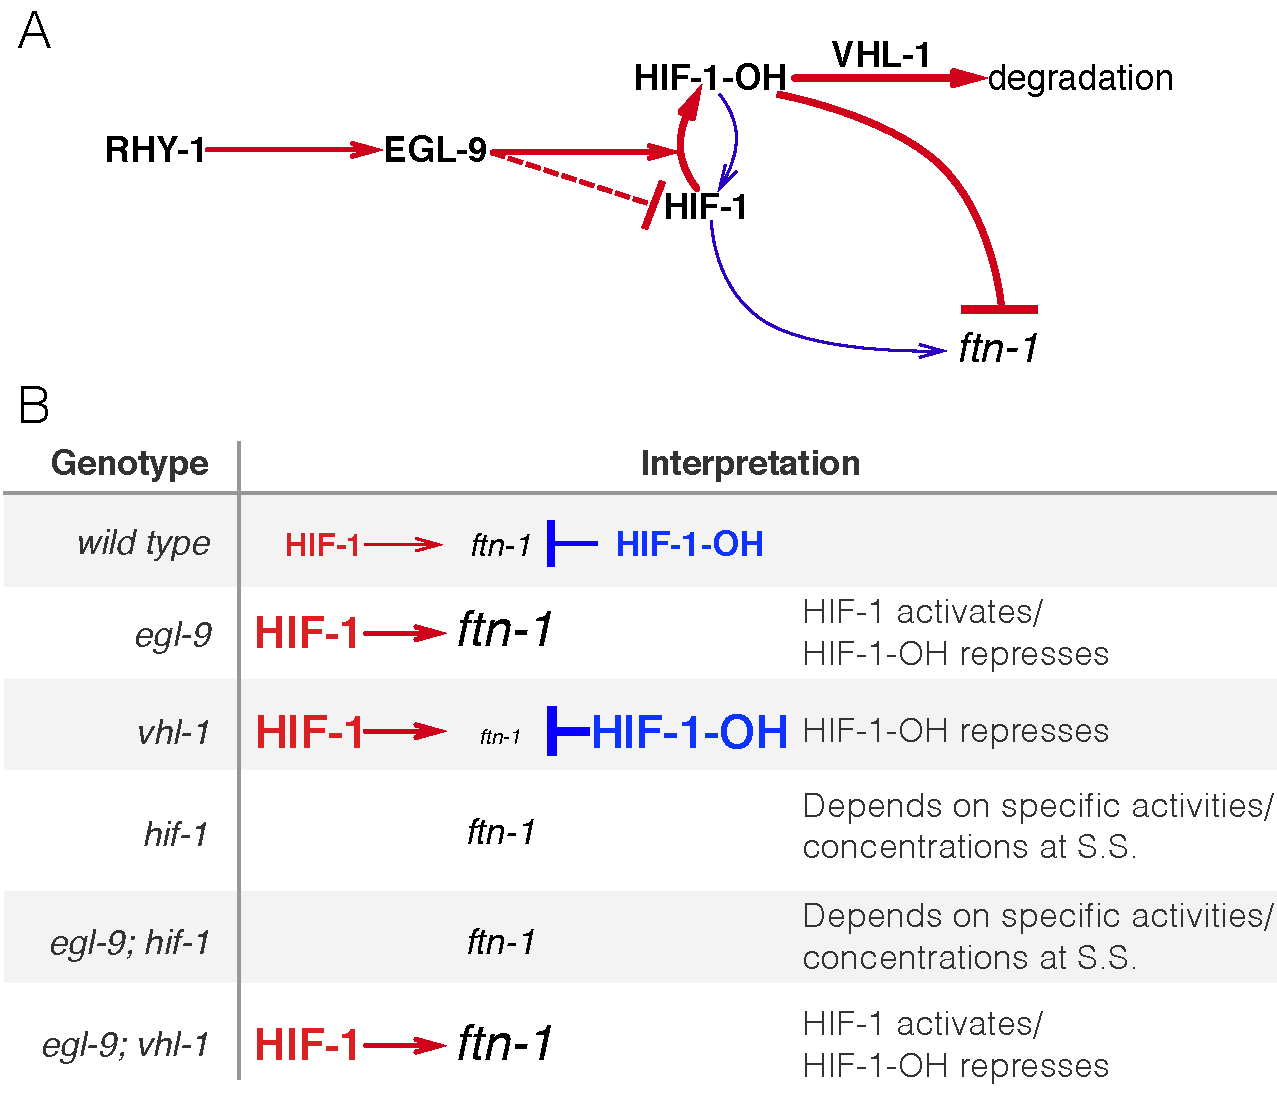
\includegraphics[width=.5\textwidth]{../figs/hif1oh_model.pdf}
  \caption{
    A hypothetical model showing a mechanism where \hifp{}-hydroxyl antagonises
    \hifp{}. \textbf{A}. Diagram showing that RHY-1 activates EGL-9. EGL-9
    hydroxylates HIF-1 in an oxygen-dependent fashion. Under normoxia, HIF-1 is
    rapidly hydroxylated and only slowly does hydroxylated HIF-1 return to its
    original state. EGL-9 can also inhibit HIF-1 in an oxygen-independent
    fashion. HIF-1 hydroxyl is rapidly degraded in a VHL-1-dependent fashion. In
    our model, HIF-1 and HIF-1 hydroxyl have opposing effects on transcription.
    The width of the arrows represents the rates under normoxic conditions.
    \textbf{B}. Table showing the effects of loss-of-function mutations on HIF-1
    and HIF-1 hydroxyl activity, showing how this can potentially explain the
    behavior of \gene{ftn-1} in each case. S.S = Steady-state.
  }
\label{fig:hif1oh_table}
\end{figure}

One parsimonious solution is to consider \hifp{} as a protein with both
activating and inhibiting states. In fact, \hifp{} already exists in two states
in \cel{}: unmodified \hifp{} and \hifp{}-hydroxyl (\hifp{}-OH). Under this
model, \hifp{}-hydroxyl antagonizes the effects of \hifp{} for certain genes
like \ftna{} or \nlp{}. Loss of \gene{vhl-1} stabilizes \hifp{}-hydroxyl. A
subset of genes that are sensitive to \hifp{}-hydroxyl will be inhibited as a
result of the increase in the amount of this species, in spite of loss of
\gene{vhl-1} function also increasing the level of non-hydroxylated \hifp{}. On
the other hand, \egl{} abgrogates \hifp{}-hydroxyl, stimulating accumulation of
\hifp{} and promoting gene activity. Whether deletion of \hif{} is overall
activating or inhibiting will depend on the relative activity of each protein
state under normoxia (see Fig.~\ref{fig:hif1oh_table}).

\hifp{}-hydroxyl is challenging to study genetically, and this may have
prevented its possible role in the hypoxia pathway from being detected. No known
mimetic mutations are available with which to study the pure hydroxylated
\hifp{} species, and mutations in the Von Hippel-Lindau gene that stabilize the
hydroxyl species also increase the quantity of non-hydroxylated \hifp{} by mass
action. Because \hifp{} is detected at low levels in cells under normoxic
conditions~\cite{Wang1993}, total \hifp{} protein levels are assumed to be so
low as to be biologically inactive.

Our data show \hifn{} genes change expression in response to loss of
\gene{hif-1} under normoxic conditions, which establishes that there is
sufficient total \hifp{} protein to be biologically active. Our analyses also
revealed that \hif{} shares positive correlations with \egl{}, \rhy{} and
\vhl{}, and that each of these genotypes also shows a secondary negative
rank-ordered expression correlation with each other. These cross-patterns
between all loss of function of inhibitors of \hifp{} and \hif{} can be most
easily explained if \hifp{}-hydroxyl is biologically active.

A homeostatic argument can be made in favor of the activity of \hifp{}-hydroxyl.
The cell must continuously monitor multiple metabolite levels. The
\gene{hif-1}-dependent hypoxia response integrates information from O$_2$,
$\alpha$-ketoglutarate and iron concentrations in the cell. One
way to integrate this information is by encoding it within the effective
hydroxylation rate of \hifp{} by \eglp{}. Then the dynamics in this system will
evolve exclusively as a result of the total amount of \hifp{} in the cell. Such
a system can be sensitive to fluctuations in the absolute concentration of
\hifp{}~\cite{Goentoro2009a}. Since the absolute levels of \hifp{} are low in
normoxic conditions, small fluctuations in protein copy-number can represent a
large fold-change in \hifp{} levels. These fluctuations would not be problematic
for genes that must be turned on only under conditions of severe
hypoxia---presumably, these genes would be associated with low affinity sites
for \hifp{}, so they are only activated when \hifp{} levels are far above
random fluctuations, such as in hypoxia.

For yet other sets of genes that must change expression in response to the
hypoxia pathway, it not be sufficiente to integrate metabolite
information exclusively via \eglp{}-dependent hydroxylation of \hifp{}. In
particular, genes that may function to increase survival in mild hypoxia may
benefit from regulatory mechanisms that can sense minor changes in environmental
conditions and which therefore benefit from robustness to transient changes in
protein copy number. Likewise, genes that are involved in iron or
$\alpha$-ketoglutarate metabolism (such as \ftna{}) may benefit from being able
to sense, accurately, small and consistent deviations from basal concentrations
of these metabolites. For these genes, the information may be better encoded by
using \hifp{} and \hifp{}-hydroxyl as an activator/repressor pair. Such circuits
are known to possess distinct advantages for controlling output in a manner that
is robust to transient fluctuations in the levels of their
components~\cite{Hart2012,Hart2013}.

Our RNA-seq data suggests that one of these atypical targets of \hifp{} may be
\rhyp{}. Although \gene{rhy-1} does not exhibit non-classical epistasis, all
genotypes containing a \hif{} mutation had increased expression levels of
\gene{rhy-1}. We speculate that if \gene{rhy-1} is controlled by both \hifp{}
and \hifp{}-hydroxyl, then this might imply that \hifp{} regulates the
expression of its pathway (and therefore itself) in a manner that is robust to
total \hifp{} levels.

\subsection*{Insights into genetic interactions from vectorial phenotypes}
Here, we have described a set of methods that can be  applied to any vectorial
phenotype studied with an appropriate experimental design. Transcriptome
profiling methods afford a lot of information, but transcriptome-wide
interpretation of the results is often extremely challenging. Each method has
its own advantages and disadvantages.

Principal component analysis is computationally tractable and clusters can often
be visually detected with ease. However, PCA can be misleading, especially when
the dimensions represented do not explain a very large fraction of the variance
present in the data. In addition, principal dimensions are the product of a
linear combination of vectors, and therefore must be interpreted with extreme
care. In this case, the first principal dimension separated genotypes that
increase \hifp{} protein levels from those that decrease it. Although PCA showed
that there is information hidden in these genotypes, it is not enough by itself
to provide biological insight.

Whereas PCA operates on all genotypes simultaneously, correlation analysis is a
pairwise procedure that measures how predictable the gene expression changes are
in a mutant given the vector of expression changes in another. Like PCA,
correlation analysis is easy and fast. Unlike PCA, the product of a correlation
analysis is a single number with a straightforward interpretation. However,
correlation analysis is sensitive to outliers. Although outliers can be
mitigated via rank-transformations, these transformations cannot remove outliers
resulting from systematic variation caused, for example, by feedback loops. Such
interactions can lead to vanishing correlations if both are equally strong.
Adequately weighted correlations could be informative for ordering genes along
pathways. A drawback of correlation analysis is that the number of pairwise
comparisons increases combinatorially.

Another way to analyze genetic interactions is via general linear models (GLMs)
that include interaction terms between two or more genes. GLMs can quantify the
genetic interactions on single genes. We and others~\cite{Dixit2016,
Angeles-Albores2016a} have used GLMs to perform epistasis analyses of
a pathway previously using transcriptomic phenotypes. GLMs are powerful, but
they generate a different interaction coefficient for each gene measured. The
large number of coefficients makes interpretation of the genetic interaction
between two mutants extremely difficult. Previous approaches~\cite{Dixit2016}
have attempted to visualize these coefficients via heatmaps.

Epistasis plots are a novel way to visualize epistasis in vectorial phenotypes.
Here, we have shown how an epistasis plot can be used to identify interactions
between two single mutants and a double mutant. In reality, epistasis plots can
be generated for any set of measurements involving a set of $N$ mutants and an
$N$-mutant genotype. Epistasis plots can accumulate an arbitrary number of
points within them, possess a rich structure that can be visualized and have
straightforward interpretations for special slope values. Epistasis plots and
GLMs are not antagonistic toward one another. Indeed, one could use a GLM to
quantify interactions at single-gene resolution, then plot the conglomerated
results in an epistasis plot instead of as a heatmap (for a non-genetic example,
see~\cite{Angeles-Albores2016a}).

Until relatively recently, the rapid generation and molecular characterization
of null mutants was a major bottleneck for genetic analyses. Advances in
genomic engineering mean that, for a number of organisms, production of mutants
is now rapid and efficient. As mutants become easier to produce, biologists are
realizing that phenotyping and characterizing the biological functions of
individual genes is challenging. This is particularly true for whole organisms,
where subtle phenotypes can go undetected for long periods of time. We have
shown that whole-animal RNA-sequencing is a sensitive method that can be
seamlessly incorporated with genetic analyses of epistasis.

\matmethods{
\subsection*{Nematode strains and culture}
Strains used were N2 wild-type Bristol,
CB5602 \gene{vhl-1}(\emph{ok161}),
CB6088 \gene{egl-9}(\emph{sa307})~\gene{hif-1}(\emph{ia4}),
CB6116 \gene{egl-9}(\emph{sa307});\gene{vhl-1}(\emph{ok161}),
JT307 \gene{egl-9}(\emph{sa307}),
ZG31 \gene{hif-1}(\emph{ia4}),
RB1297 \gene{rhy-1}(\emph{ok1402}).
All lines were grown on standard nematode growth media (NGM) plates seeded with
OP50 \ecol{} at 20\degree{}C~\cite{Brenner1974}.

\subsection*{RNA isolation}
Lines were synchronized by harvesting eggs via sodium hypochlorite treatment and
subsequently plating eggs on food. Worms were staged and based on the time after
plating, vulva morphology and the absence of eggs. 30--50 non-gravid young
adults were picked and placed in 100 $\mu$L of TE pH 8.0 (Ambion AM 9849) at
4\degree{}C in $0.2$ mL PCR tubes. Worms were allowed to settle or spun down by
centrifugation and $\sim 80~\mu$L of supernatant removed before flash-freezing in
liquid N2. These samples were digested with Proteinase K (Roche Lot No. 03115
838001 Recombinant Proteinase K PCR Grade) for 15min at 60\degree{} in the
presence of 1\% SDS and 1.25 $\mu$L RNA Secure (Ambion AM 7005). RNA samples were
then taken up in 5 Volumes of Trizol (Tri Reagent Zymo Research) and processed
and treated with DNase I using Zymo MicroPrep RNA Kit (Zymo Research Quick-RNA
MicroPrep R1050). RNA was eluted in RNase-free water stored at -80\degree{}C.
Samples were analyzed using a NanoDrop (Thermo Fisher) for impurities, Qubit for
concentration and then analyzed on an Agilent 2100 BioAnalyzer (Agilent
Technologies). Replicates were selected that had RNA integrity numbers (RIN)
equal or greater than 9.0 and showed no evidence of bacterial ribosomal bands,
except for the ZG31 mutant where one of three replicates had a RIN of 8.3.

\subsection*{Library preparation and sequencing}
10ng of quality checked total RNA from each sample was reverse-transcribed into
cDNA using the Clontech SMARTer Ultra Low Input RNA for Sequencing v3 kit
(catalog \#634848) in the SMARTSeq2 protocol~\cite{Picelli2014}.  RNA was
denatured at 70\degree{}C for 3 minutes in the presence of dNTPs, oligo dT
primer and spiked-in quantitation standards (NIST/ERCC from Ambion, catalog
\#4456740).  After chilling to 4\degree{}C, the first-strand reaction was
assembled using the LNA TSO primer described in Picelli et
al~\cite{Picelli2014}, and run at 42\degree{}C for 90 minutes, followed by
denaturation at 70\degree{}C for 10 minutes.  The entire first strand reaction
was then used as template for 13 cycles of PCR using the Clontech v3 kit.
Reactions were cleaned up with 1.8x volume of Ampure XP SPRI beads (catalog
\#A63880) according to the manufacturer’s protocol.  After quantification using
the Qubit High Sensitivity DNA assay, a 3ng aliquot of the amplified cDNA was
run on the Agilent HS DNA chip to confirm the length distribution of the
amplified fragments.  The median value for the average cDNA lengths from all
length distributions was 1,076bp.  Tagmentation of the full length cDNA for
sequencing was performed using the Illumina/Nextera DNA library prep kit
(catalog \#FC-121--1030). Following Qubit quantitation and Agilent BioAnalyzer
profiling, the tagmented libraries were sequenced. Libraries were sequenced on
Illumina HiSeq2500 in single read mode with the read length of 50nt to an
average depth of 15 million reads per sample following manufacturer's
instructions. Base calls were performed with RTA 1.13.48.0 followed by
conversion to FASTQ with bcl2fastq 1.8.4. Spearman correlation of the estimated
counts for each genotype showed that every pairwise correlation within genotype
was $0.9$.

\subsection*{Read alignment and differential expression analysis} We used
Kallisto~\cite{Bray2016} to perform read pseudo-alignment and performed
differential analysis using Sleuth~\cite{Pimentel2016}. We fit a general linear
model for a transcript $t$ in sample $i$:
\begin{equation}
  y_{t,i} = \beta_{t, 0} + \beta_{t, genotype}\cdot{}X_{t, i} +
  \beta_{t, batch}\cdot{}Y_{t, i} + \epsilon_{t, i}
\end{equation}
where $y_{t, i}$ was the logarithm transformed counts; $\beta_{t, genotype}$ and
$\beta_{t, batch}$ were parameters of the model, and which could be interpreted
as biased estimators of the log-fold change; $X_{t, i}, Y_{t, i}$ were indicator
variables describing the conditions of the sample; and $\epsilon_{t, i}$ was the
noise associated with a particular measurement.

\subsection*{Genetic Analysis, Overview}
The processed data were analyzed using Python 3.5. We used the Pandas,
Matplotlib, Scipy, Seaborn, Sklearn, Networkx, PyMC3, and TEA
libraries~\cite{McKinney2011,Oliphant2007,
Pedregosa2012,Salvatier2015,VanDerWalt2011,Hunter2007,Angeles-Albores2016,Waskom}.
Our analysis is available in Jupyter Notebooks~\cite{Perez2007}. All code and
processed data are available at
\url{https://github.com/WormLabCaltech/mprsq} along with version-control
information. Our Jupyter Notebook and interactive graphs for this project can be
found at \url{https://wormlabcaltech.github.io/mprsq/}. Raw reads were deposited
in the Short Read Archive under the study accession number SRP100886.

\subsection*{Weighted correlations}
Pairwise correlations between transcriptomes were calculated by identifying the
set of DEGs common to both transcriptomes under
analysis. DEGs were rank-ordered according to their regression coefficient,
$\beta$. Bayesian robust regressions were performed using a Student-T
distribution using the PyMC3 library~\cite{Salvatier2015}
(\texttt{pm.glm.families.StudenT} in Python). If the correlation had an average
value $>1$, the average correlation coefficient was set to 1.
Weights were calculated as the proportion of genes that were inliers to a
regression divided by the total number of DEGs present
in either mutant.

\subsection*{Epistatic analysis}
The epistasis coefficient between two null mutants \gene{a} and \gene{b} was
calculated as:
\begin{equation}
  s(a, b) = \frac{\beta_{a,b} - \beta_a - \beta_b}{\beta_a + \beta_b}
\label{eq:epistasis_coef}
\end{equation}

Null models for various epistatic relationships were generated by sampling the
single mutants in an appropriate fashion. For example, to generate the
distribution for $a^- = a^-b^-$, we substituted $\beta_{a, b}$ with $\beta_a$
and bootstrapped the result.

To select between theoretical models, we implemented an approximate Bayesian
Odds Ratio. We defined a free-fit model, $M_1$, that found the line of best fit
for the data:
\begin{equation}
  P(\alpha~|M_1, D) \propto \prod_{(x_i, y_i, \sigma_i)\in D}
  \exp{
       [\frac{{(y_i - \alpha\cdot x_i)}^2} % numerator
            {2\sigma_i^2}] % denominator
      } \cdot {(1+\alpha^2)}^{-3/2},
  \label{eq:free_model}
\end{equation}
where $\alpha$ was the slope to be determined, $x_i, y_i$ are the
of each point, and $\sigma_i$ was the standard
error associated with the y-value. We used equation~\ref{eq:free_model} to
obtain the most likely slope given the data, $D$, via minimization
(\texttt{scipy.optimize.minimize} in Python). Finally, we approximated the odds
ratio as:

\begin{equation}
  OR = \frac{
  P(D~|\alpha^*, M_1)\cdot {(2\pi)}^{1/2}\sigma_{\alpha^*} % numerator
  }{P(D~| M_i)}, % denominator
\end{equation}
where $\alpha^*$ was the slope found after minimization, $\sigma_\alpha^*$ was the
standard deviation of the parameter at the point $\alpha^*$ and $P(D~|M_i)$ was
the probability of the data given the parameter-free model, $M_i$.

\subsection*{Enrichment analysis}
Tissue, Phenotype and Gene Ontology Enrichment Analysis were carried out using
the WormBase Enrichment Suite for Python~\cite{Angeles-Albores106369,
Angeles-Albores2016}.

} % end methods

\showmatmethods{} % Display the Materials and Methods section

\acknow{
This work was supported by HHMI with whom PWS is an investigator and by the
Millard and Muriel Jacobs Genetics and Genomics Laboratory at California
Institute of Technology. All strains were provided by the CGC, which is funded
by NIH Office of Research Infrastructure Programs (P40 OD010440). This article
would not be possible without help from Dr.\ Igor Antoshechkin who performed all
sequencing. We thank Hillel Schwartz, Jonathan Liu, Han Wang, and Porfirio
Quintero and Erich Schwarz for their advice, support and conversations
throughout this project. }

\showacknow{} % Display the acknowledgments section

% \pnasbreak splits and balances the columns before the references. % If you see
% unexpected formatting errors, try commenting out this line % as it can run into
% problems with floats and footnotes on the final page.
% \pnasbreak{}

% Bibliography
\bibliography{citations}

\end{document}
